% AI Shield v2 replacement text for Sections 5, 6, 9, and Appendix A.
% Generated from results_v2.json. Percentages are rounded to two decimals.

\section{Results}

Table~\ref{tab:v2-results} reports binary results with both \textsc{Suspicious} and
\textsc{Scam} treated as a positive warning.  The held-out Nazario set contains
200 phishing and 200 legitimate messages.  AI Shield v2.1 detected 189 phishing
messages and incorrectly warned on nine legitimate messages.  Recall increased
from 10.67\% in v1 to 94.50\%, while specificity remained above the prespecified
90\% target at 95.50\%.  The corresponding 95\% percentile bootstrap intervals
(1,000 resamples) were 91.28--97.62\% for recall, 92.67--98.35\% for
specificity, 92.57--98.38\% for precision, and 92.80--97.07\% for F1.

\begin{table}[ht]
\centering
\caption{AI Shield v2 evaluation. Synthetic scam sets contain positives only;
therefore specificity is undefined for those rows.}
\label{tab:v2-results}
\begin{tabular}{lrrrrrr}
\hline
Dataset & $n$ & TP & TN & FP & FN & Recall \\
\hline
Nazario held-out & 400 & 189 & 191 & 9 & 11 & 94.50\% \\
Hindi/Hinglish UPI scams (synthetic) & 200 & 200 & -- & -- & 0 & 100.00\% \\
English banking scams (synthetic) & 200 & 200 & -- & -- & 0 & 100.00\% \\
\hline
\end{tabular}
\end{table}

The synthetic domain-shift test replaces the v1 UCI generic-spam evaluation.
All 200 Hindi/Hinglish UPI scams and all 200 English banking scams were warned on.
These template-generated samples measure coverage of the specified scenarios;
they are not independent evidence of performance on naturally occurring scams.
An additional negative-control regression set included 200 synthetic benign
controls per language. The revised detector correctly cleared all 400, including
receipts and safety advice such as ``never share an OTP.'' Because these cases were
used to guide changes, the perfect synthetic score is not an independent estimate
of real-world specificity or negation understanding.

Median detector latency was 4.67\,ms on held-out Nazario messages and 1.34\,ms on
the synthetic suite; the Nazario 95th percentile was 19.62\,ms.  Both medians meet
the under-5\,ms target.  These measurements cover local detector execution only,
not popup rendering, page extraction, browser scheduling, or hardware variation.

\begin{figure}[ht]
\centering
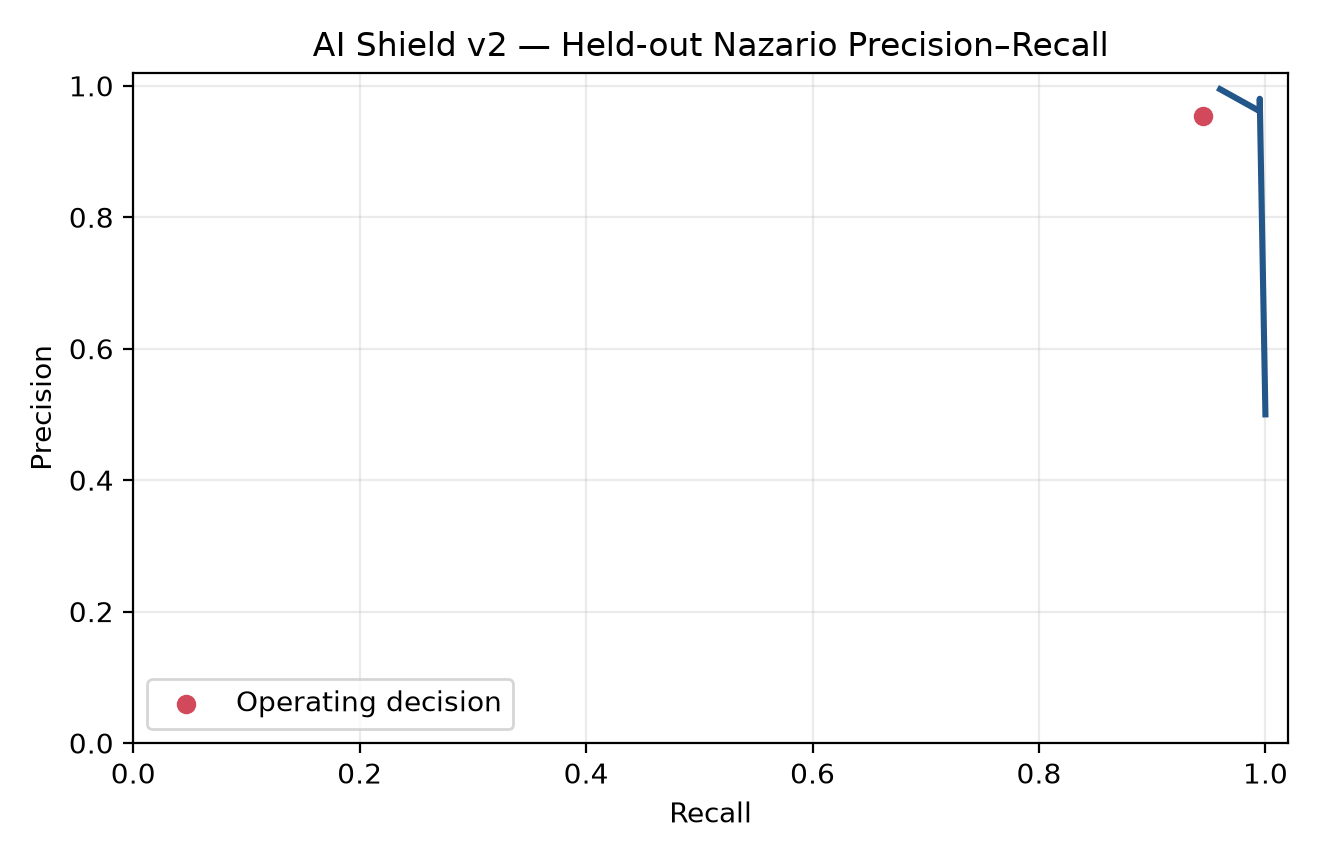
\includegraphics[width=.78\linewidth]{figure_pr_curve.png}
\caption{Precision--recall curve on the held-out Nazario split.}
\label{fig:pr-v2}
\end{figure}

\begin{figure}[ht]
\centering
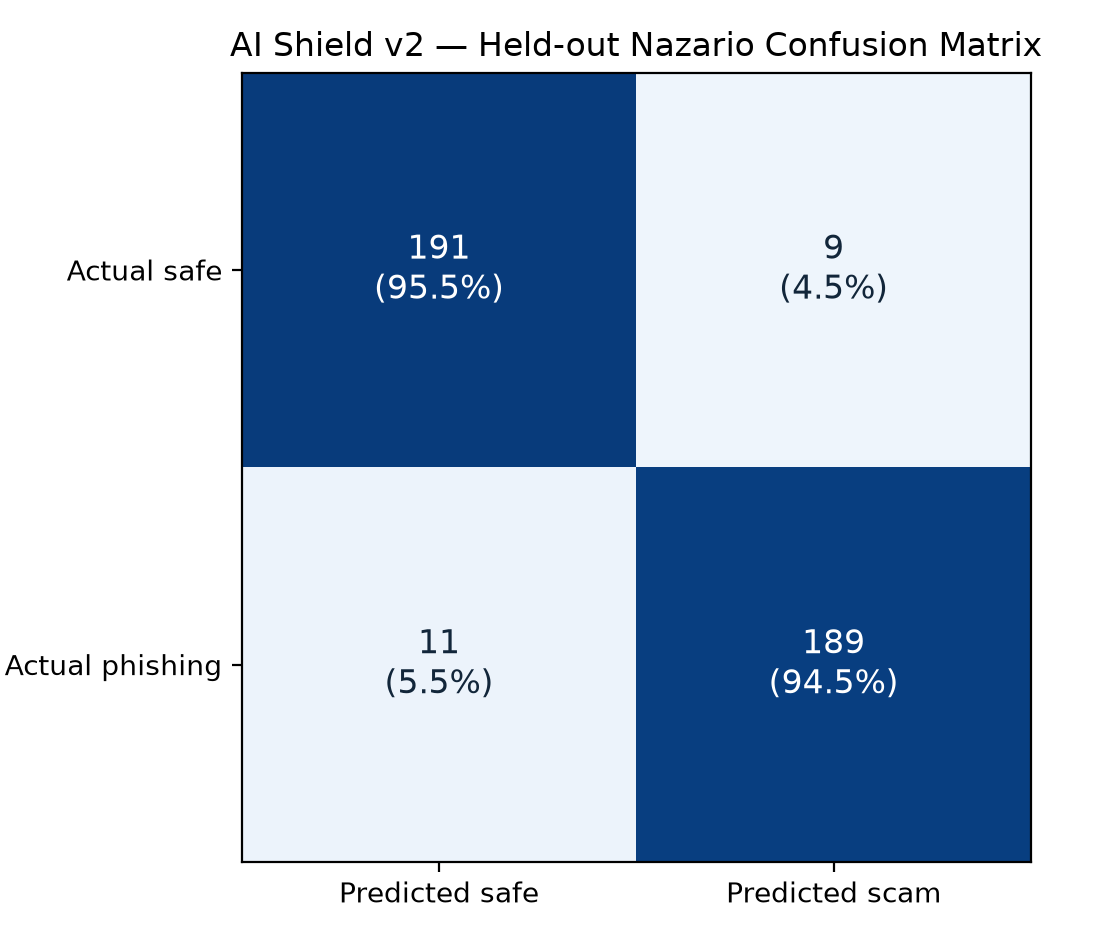
\includegraphics[width=.72\linewidth]{figure_cm_v2.png}
\caption{Held-out Nazario confusion matrix with row percentages.}
\label{fig:cm-v2}
\end{figure}

\section{Discussion}

Retraining the embedded multinomial Naive Bayes model on a deduplicated,
phishing-specific sample removed the main v1 recall failure on the deterministic
held-out split.  The compact 130\,KB artifact remains suitable for offline
Manifest V3 packaging.  Unicode tokenization adds Devanagari support, and explicit
rules now cover IP-address URLs, punycode, shorteners, suspicious top-level
domains, and known-brand display-name/domain mismatches.  Scoring remains local,
bounded to 0--100, with thresholds of 35 and 70 shared by the web and extension.

The results still reject the claim that the detector is production-ready.
The high held-out recall may reflect random-split similarity,
historical-corpus artifacts, sender or URL shortcuts, and residual campaign-level
near duplicates.  Only exact normalized duplicates were removed; no temporal or
campaign-grouped split was available.  The synthetic scam result is also expected
to be optimistic because the templates deliberately instantiate detector-visible
features.  The prior false alarms on safety reminders motivated a narrow
context rule; naturally occurring negatives are still needed to test its limits.

Sender-domain mismatch is evaluated only when sender text is present in the input.
The current extension extracts rendered page text and does not obtain authenticated
mail headers such as SPF, DKIM, or DMARC results.  URL checks inspect lexical form
without resolving redirects, querying reputation services, or visiting links,
which preserves the local-only privacy design but limits coverage.  Image-only
lures, QR payloads not represented as text, obfuscation, new languages, and targeted
spear phishing remain outside the demonstrated evidence.

A \textsc{Safe} result therefore continues to mean ``No suspicious patterns found,
but verify via official channel.''  The detector should remain advisory.  A stronger
evaluation should freeze a temporally newer external corpus, group related campaigns
before splitting, manually audit false positives and false negatives, and test
calibration and user decisions with preregistered procedures.

\section{Conclusion and Future Work}

AI Shield v2 demonstrates that a compact embedded model can substantially improve
held-out phishing recall while preserving offline inference, the \texttt{activeTab}
and \texttt{scripting} permission boundary, and millisecond-scale median latency.
On the deterministic Nazario split it achieved 94.50\% recall, 95.50\% specificity,
and 95.45\% precision.  It also warned on every generated Hindi/Hinglish UPI and
English banking scam in the scenario suite.

These measurements do not justify deployment as an autonomous security control.
The test-guided synthetic benign set, random rather than temporal corpus split, and
absence of authenticated sender metadata leave material uncertainty.  Future work
should add campaign-grouped and temporal external validation, negation-aware text
features, calibrated probabilities, multilingual natural samples, OCR/QR evaluation,
and a user study of whether explanations improve independent verification without
creating false reassurance.

\section*{Appendix A: Reproducibility}

The v2 pipeline uses Python's standard library for preparation, metrics, and
bootstrap resampling, Matplotlib for figures, and Node.js for executing the same
shared detector used by the web application and extension:
\begin{verbatim}
python3 research/train_v2.py
node research/evaluate_v2.mjs
MPLCONFIGDIR=/tmp/matplotlib-ai-shield python3 research/analyze_v2.py
\end{verbatim}
The deterministic seed is 20260915.  The source SHA-256 values are
\texttt{afef69828165619ced6661ca14a95444a1db82c7b25ae9c2619bbbb108844a44}
for \texttt{Nazario\_5.csv} and
\texttt{7d039a24a6083ed9ef0f806ebad56bbb976e3aeb8de05669173bfdc4996c239d}
for the extracted UCI file.  No exact normalized Nazario/UCI overlaps were found.
The four UCI-versus-embedded-corpus overlaps reported in v1 are eliminated because
v2 does not train on that 40-message corpus.  The generated model SHA-256 is
\texttt{3476e78c882d9d84e7e3cec3114902bb509fda1f95d182b492acd2c6a36d8b30}.
